
\documentclass[sigchi]{acmart}

\settopmatter{printacmref=false, printccs=true, printfolios=true}
%%
%% \BibTeX command to typeset BibTeX logo in the docs
\AtBeginDocument{%
  \providecommand\BibTeX{{%
    \normalfont B\kern-0.5em{\scshape i\kern-0.25em b}\kern-0.8em\TeX}}}

%% Rights management information.  This information is sent to you
%% when you complete the rights form.  These commands have SAMPLE
%% values in them; it is your responsibility as an author to replace
%% the commands and values with those provided to you when you
%% complete the rights form.
\setcopyright{none}
%\copyrightyear{none}
\acmYear{2021}
\acmDOI{}

%% These commands are for a PROCEEDINGS abstract or paper.
\acmConference[Technical Report]{May}{{\today}}{Cologne, Germany}
\acmBooktitle{}
\acmPrice{}
\acmISBN{}
\acmDOI{}

\usepackage{float}
\usepackage{subfig}
\usepackage[english]{babel}
\begin{document}

\title{The Impact of the Avatar Representation on Team Trust and Effectiveness in a Shared Virtual Environment}

\author{Hannes Hinrichs}
\email{hhinrich@smail.th-koeln.de}
\affiliation{%
  \institution{TH-Köln}
  \city{Cologne}
  \country{Germany}
}

\begin{abstract}
This paper investigates the impact of the avatar representation on team trust and effectiveness in a shared virtual environment. The first question addressed in this paper is whether an inverse-kinematic humanlike representation or an abstract non-humanlike representation is more effective in generating trust in a newly formed virtual team. Furthermore, it is analyzed whether the trust formed by the different representations influences the effectiveness of a virtual team. To answer these questions, a quantitative study has been conducted, in which different participants in a three-person team performed a collaborative task in a shared virtual environment. No significant differences in effectiveness were found among the teams. The results of the study also show that in the three-person team significantly more trust was built with non humanlike avatars. Furthermore, with non-humanlike avatars a significant correlation between the cognitive trust formed and team effectiveness was found. The results suggest that the simplicity of a non-humanlike avatar in a newly formed team in a shared virtual environment can be effective in creating a trusting work environment.
\end{abstract}

\keywords{Virtual-Reality, Trust, Team Formation, Virtual Teams, Avatar}

%% A "teaser" image appears between the author and affiliation
%% information and the body of the document, and typically spans the
%% page.
\begin{teaserfigure}
  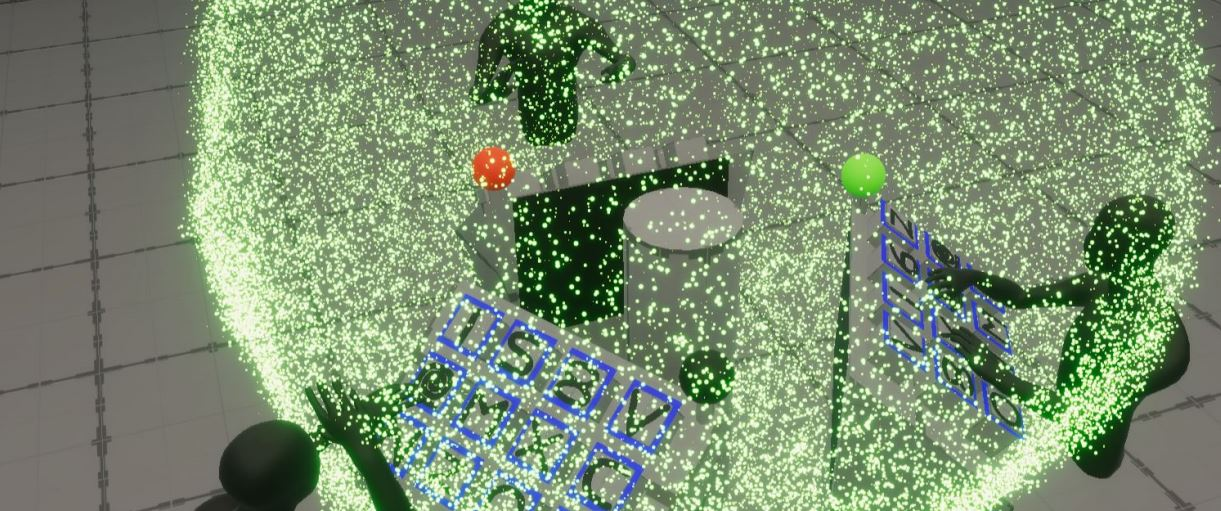
\includegraphics[width=\textwidth]{Abbildungen/RoundSuccsessful2}
  \caption{This figure represents the developed Shared-Virual-Environment with the participants in front of their podiums. A green sphere appears clearly visible when a round is successfully completed.}
  \Description{This figure represents the developed Shared-Virual-Environment. The green sphere appears clearly visible for all participants when a round is successfully completed.}
  \label{fig:teaser}
\end{teaserfigure}

%%
%% This command processes the author and affiliation and title
%% information and builds the first part of the formatted document.
\maketitle

\section{INTRODUCTION}
With advancing technological development, digital communication is becoming more and more central. Companies around the world have long relied on overcoming spatial and temporal boundaries.
New generations of social networking systems are being created on the premise of improving communication to remote individuals.
Fields of application include mobile and internet communication, FOIP/VOIP teleconferencing, and 3D social virtual environments.
All these technologies share the goal of enhancing social presence, allowing users to gain some degree of insight and the \textit{cognitive and affective states} of the interaction partner \citep{biocca2002defining}.
Employees in a company are often scattered across the globe, yet many companies still want their teams to be effective \citep{jarvenpaa1999communication}. \textit{Virtual teams} can provide a remedy here. 
Before the coronavirus pandemic, in Q2 2020, 4\% of all employees in Germany worked from home. This percentage has risen to 24\% over the course of the year - as of 01.01.2021 - and theoretically, 80\% of employees could work from home. \citep{statistaCorona2020}. As a result of this development, companies inevitably have had to look at how virtual teams work.
When a virtual team meets in a virtual reality environment, avatars can be used to represent the individual. These avatars are used to interact and communicate with other participants in the shared virtual environment.
\textit{Virtual teams} are often short-lived, which creates a deficit in the \textit{trust formed} with team members.
Working in a geographically separated team that does not trust each other or does not work together properly inhibits its performance. \citep{huang1998supporting}; \citep{turoff1993distributed}. This paper aims to better understand the construct of trust in the virtual world and how to deal with it in order to work more effectively in a virtual team.
The goal of the conducted study was to find out which type of representation builds more trust in a virtual team. The focus was on the two avatar conditions \textit{humanlike} and \textit{non-humanlike}, in order to analyze whether there is a correlation between the \textit{cognitive trust} formed in the team and the \textit{team effectiveness} with the use of different avatar representation types during collaboration.
In addition, another focus was on the general propensity to trust of individual trial participants to investigate whether the \textit{general propensity to trust} has an influence on the \textit{team effectiveness} and the \textit{cognitive trust} with respect to the different avatar representations. For this purpose, a three-person team, whose members did not know each other, competed in a collaborative task in a shared virtual environment.

\section{RELATED WORK}
This section provides an overview of the topic of trust and teams.
\subsection{TRUST}
The most commonly used definition of trust comes from Meyer et al. \citep[p. 712]{mayer1995integrative}. They define trust as
\begin{quote} \grqq{}the willingness of a party to be vulnerable to the actions of another party based on the expectation that the other will perform a particular action important to the trustor, irrespective of the ability to monitor or control that other party\grqq{} \citep[p. 712]{mayer1995integrative}.\end{quote}

Trust is not considered static and one-sided. A person can not only \textit{trust} or \textit{not trust}. Trust is a dynamic construct that changes over time. It can be divided into a formation, a stabilization and a decreasing phase \citep{rousseau1998not}.

During the early phase of trust building, it is decided whether a relationship will be maintained or not. Subconsciously, a feeling of confidence and security or a feeling of tension, doubt and skepticism towards the interaction partner is formed.
It does not matter whether the decision is made to trust someone or not. The strength of the positive or negative subconscious sense of trust influences the effectiveness of the collaboration. Trust can make it easy or difficult to work with another person and to achieve goals in a group or team \citep{bigley1998straining}.

The initial phase of trust formation affects the \textit{cognitive} trust, which has a strong influence on the developing trust model about a person.
Opinions and assumptions formed early on thus strongly shape future opinions about the trustee \citep{baldwin1992relational}.

Many psychologists studying trust now assume that \textit{interpersonal} trust consists of a two-dimensional construct \citep{johnson2005cognitive}; \citep{cook1980new}. Thus, Mooradian et al. consider that trust is viewed as a \textit{trait} or as a \textit{state} \citep{mooradian2006trusts}.

\subsubsection{TRUST AS A TRAIT}
Trust as a trait reflects a person's attitude toward trust. This attitude toward trust is long-lasting and is not quickly built up or broken down. It is the fundamental level of trust that a person brings into a new interpersonal relationship \citep{couch1996assessment}. 

\textit{General trust} implies that most persons can be trusted, or that in the case of general distrust, persons can not be trusted \citep{stolle2002trusting}.

The \textit{general trust} is not situation-dependent, but represents a longer-term constant, based on the baseline of trust of a person. In this context, it is composed of the individual characteristic of an individual person's propensity to trust, as well as the basic mood towards people in general \citep{couch1996assessment}.

\subsubsection{TRUST AS A STATE}
If trust is viewed as \textit{a state}, it is considered that this state can change over time \citep{mayer1995integrative}.

According to the study by Lewis et al. \citep[p. 970-971]{lewis1985trust}, \textit{trust as a state} is based on
\begin{quote} \grqq{}a cognitive process which discriminates among persons and institutions that are trustworthy, distrusted, and unknown. In this sense, we cognitively choose whom we will trust in which respects and under which circumstances, and we base the choice on what we take to be "good reasons", constituting evidence of trustworthiness\grqq{} \citep[p. 970]{lewis1985trust}.\end{quote}

\textit{Cognitive trust} is based on a logic we define rather than an emotional component. It can be established in the short term and is easily vulnerable to external influences \citep{lewis1985trust}. 

Thus, individual \textit{cognitive trust} is based on the conviction in the abilities or reliability of another \citep{mcallister1995affect}.

\subsection{VIRTUAL TEAMS}
A Team is defined as \begin{quote}\grqq{}a small number of people with complementary skills who are equally committed to a common purpose, goals, and working approach\grqq{} \citep[p. 718]{zenun2007effects}. \end{quote}

According to Schweitzer et al. \citep{schweitzer2010conceptualizing}, \textit{virtual teams} share many characteristics of traditional \textit{teams}, but have a virtual component.
They become into being due to communication technology and work spatially separated, across borders, and asynchronously.

The challenge of a \textit{virtual team} arises from the different cultures, distances and time zones of the team members. If the members of a \textit{virtual team} trust each other, the disadvantage of different cultures, distances and time zones can become an advantage. Cultural diversity is promoted and new patterns of behavior are acquired, fostering new, creative ways of working. Through these factors it is possible to work and think more innovatively \citep[p. 67-74]{dyer1995team} \citep{milliken1996searching}.

Virtuality is viewed as a continuum, where each team has some degree of virtuality. This continuum ranges from face-to-face to communicating entirely via communication technology \citep{martins2004virtual} (see \textit{Figure \ref{virtualTeamsVirtuality}}).

\begin{figure}[h]
  \centering
 	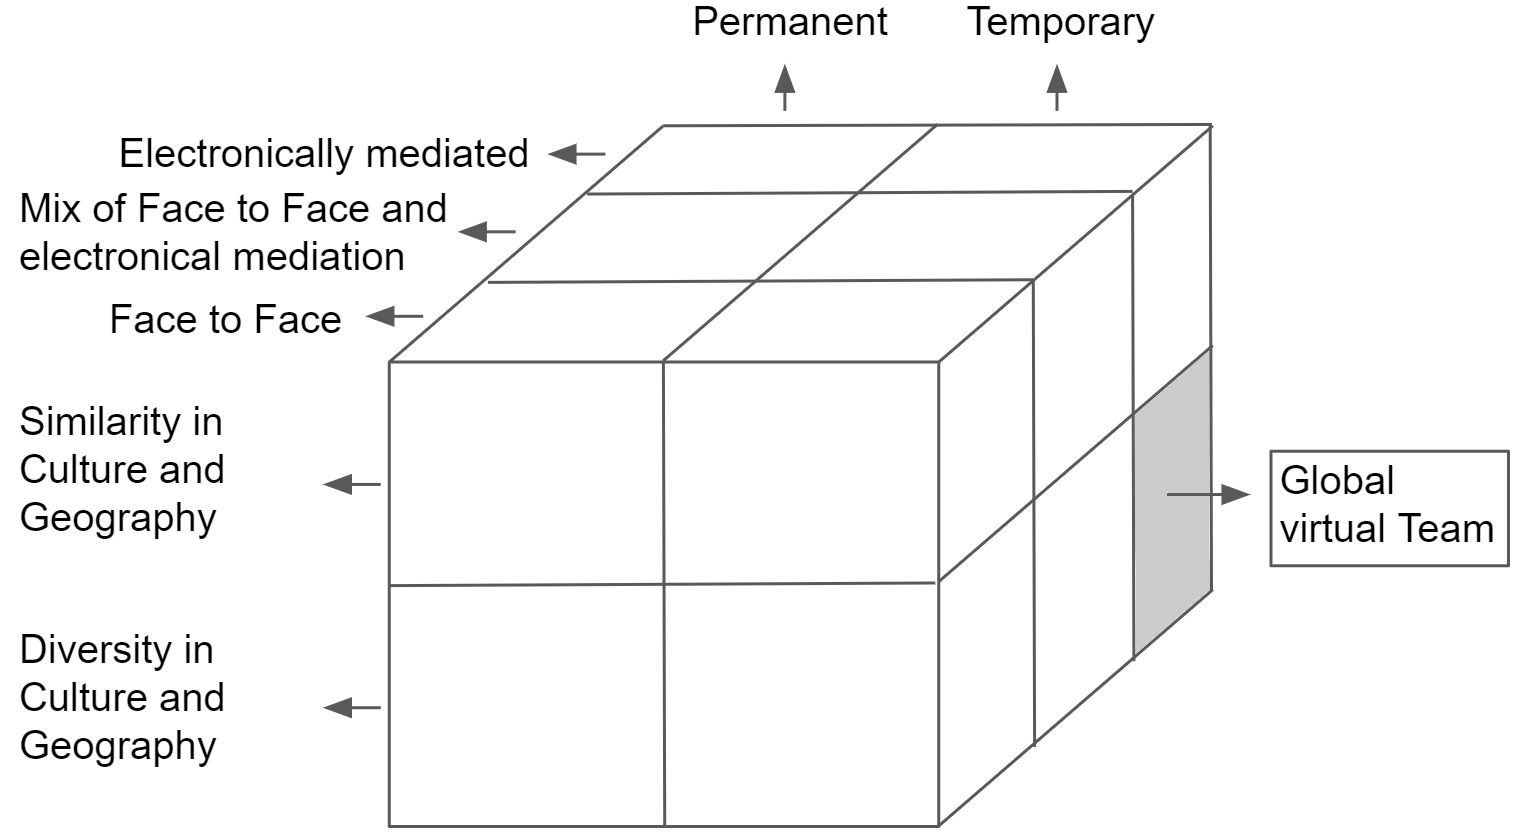
\includegraphics[width=\linewidth]{Abbildungen/Global-Virtual-Team.jpg}	
			\caption[Virtuality of a virtual team]{Degree of virtuality that a team must reach to be considered a \textit{virtual team} \citep{jarvenpaa1999communication}.}
			\label{virtualTeamsVirtuality}
\end{figure}

Members of a \textit{virtual team} have fewer to no opportunities to see each other in person, interact or resolve conflicts, unlike traditionally formed teams. Respect and trust are the basic building blocks of a \textit{virtual team}. The effectiveness of a team is a direct consequence of this \citep{ren2007applying}.

\subsection{VIRTUAL TEAMS AND TEAM EFFECTIVENESS}
\textit{Team effectiveness} is the ability of a team to interact and support each other in a way that achieves a previously defined goal of the team. Because many external factors can contribute to the achievement of the goal, it is important that the team always have a focus on its \textit{team effectiveness} \citep{salas2005there}.

According to Cohen et al. \citep{cohen1997makes}, team effectiveness can be measured by a team's performance effectiveness (productivity, efficiency), attitudes toward the team (satisfaction, commitment, and trust), and by behavioral outcomes (fluctuation, turnover, safety). 

Thus, the measurement of team effectiveness can be divided into objective as well as subjective data. Objective data varies depending on the team and can be, for example, the number of completed tasks or the number of customer complaints. Subjective data is collected via questionnaires and aims to determine the perceived team effectiveness or the effectiveness of individual team members. Perceived workload, perceived quality of work, and perceived productivity are also used to measure team effectiveness. However, all of these effectiveness measures can have different weights from team to team and standard of measurement can be defined \citep{pina2008teams}. 

Furthermore, it is assumed that effectiveness in groups can be measured by the outcomes produced by the group as a whole \citep{guzzo1996teams}. 

Schweitzer et al. \citep{schweitzer2010conceptualizing} assume that traditionally formed teams are more effective than \textit{virtual teams} and that \textit{team effectiveness} decreases the higher the degree of virtuality.
This assumption is also shared by Becker et al. According to them, the exchange of information content and the building of trust suffers due to increasing virtuality and the same effectiveness as in a face-to-face team cannot be achieved \citep{handke2019alles}.

Previous studies have found positive correlations \citep{davis2000trusted}, no correlations \citep{hertel2004managing}, and negative correlations \citep{dirks1999effects} between \textit{trust} and \textit{team effectiveness} in \textit{virtual teams}.

Despite the contradictory results of these studies, the general opinion can be described as trust having a positive influence on \textit{team effectiveness} \citep{de2016trust}. 
Trust in your team helps to block out your own uncertainties in order to work more self-confident and effectively \citep{en2010does}. Furthermore, existing trust in your team creates a greater interest in the team members, which unlocks synergy effects and enables more direct and effective interactions \citep{dirks1999effects}. 

\subsection{AVATARS AND TRUST}
George et al. \citep{george2018trusting} analyze in their research, whether more trust can be established with humanlike or robotic avatars in a shared virtual environment. They find no significant difference in trustworthiness. However, a greater sense of commonality can be found when interacting with a humanlike avatar.

Riedl et al. \citep{riedl2014trusting} conducts a study on trust-building among humans compared to avatars with humanlike faces. They find that people find it easier, to trust a real person rather than an avatar with a humanlike face. According to them, trust is built between humans at the same rate as between humans and avatars.
This assumption was also confirmed by Bente et al. \citep{bente2004social}. They find that in a shared virtual environment less \textit{cognitive trust} is built towards avatars compared to face-to-face, telephone and chat communication.

\section{METHOD}
An \textit{A/B}-Test in combination with an inductive quantitative research design was chosen.
Group A was assigned the condition humanlike, while group B was assigned the condition non-humanlike (\textit{Figure \ref{Avatars}}). Participants were randomly assigned to groups and conditions. 

The analysis in this study was conducted at different levels.
Since the participants work as a team and different teams have different conditions, some correlations and differences were analyzed on \textit{condition level} and some were analyzed on \textit{team level}.

The \textit{individual level} is about an individual person, while the \textit{condition level} distinguishes between the conditions \textit{humanlike} and \textit{non-humanlike}.

The condition level can be divided into teams of 3 persons each. This division is called \textit{team level} and makes it possible, to make assumptions about the whole team. 
The \textit{Figure \ref{DifferentLevels}} shows the hierarchy of the different levels.

\begin{figure}[h]
  \centering
 		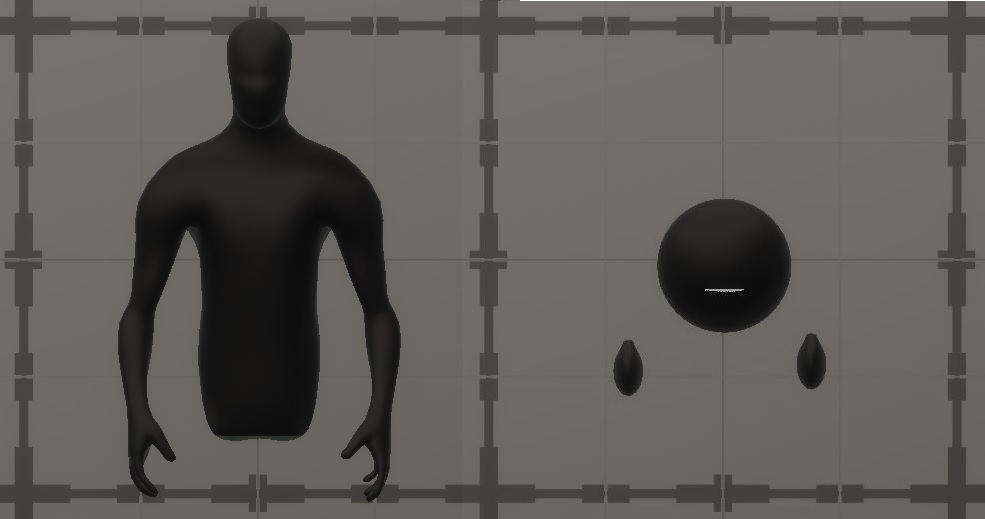
\includegraphics[width=0.60\linewidth]{Abbildungen/Avatars.JPG}
			\caption[The avatars]{This figure shows the avatars used during the experiment. Left: \textit{humanlike} avatar and right: \textit{non-humanlike} avatar.}
			\label{Avatars}
\end{figure}	

\begin{figure}[h]
  \centering
 		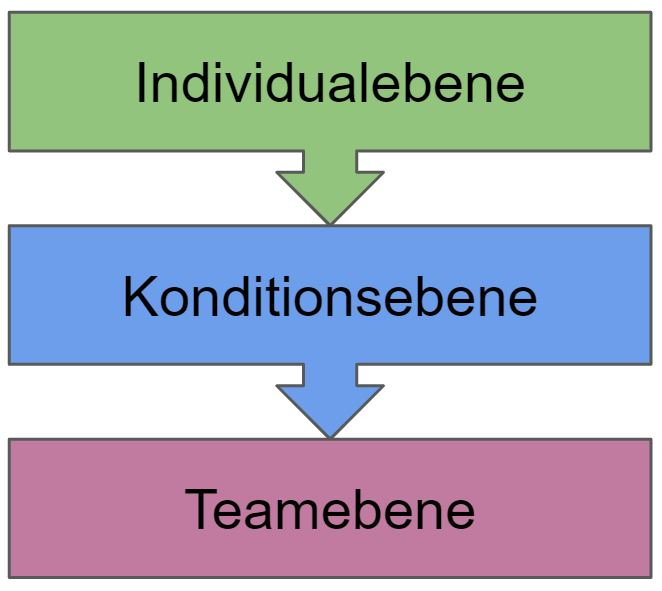
\includegraphics[width=0.5\linewidth]{Abbildungen/DifferentLevels.JPG}	
			\caption[The hierarchy levels]{The hierarchy of individual level, condition level and team level.}
			\label{DifferentLevels}
\end{figure}	
	
Using a self-constructed theory-based framework (see \textit{Figure \ref{Versuchshypothesen}}), the following hypotheses were formulated :

\textbf{H1}: The mean values of the obtained \textit{cognitive trust scores} are significantly different from each other between the \textit{humanlike} and \textit{non-humanlike} conditions.

\textbf{H2}: The higher the achieved \textit{general trust score} of a person, the higher the achieved \textit{cognitive trust score} of a person.

\textbf{H3}: The correlation between the \textit{cognitive trust score of teams} and the \textit{team effectiveness} with the condition \textit{humanlike} is stronger than the correlation of teams with the condition \textit{non-humanlike}.

\textbf{H4}: The mean values of the obtained \textit{team effectiveness scores} are significantly different from each other between the \textit{humanlike} and \textit{non-humanlike} conditions.

\textbf{H5}: The correlation between the \textit{general trust score of a team} and the \textit{team effectiveness} with the condition \textit{humanlike} is stronger than that of teams with the condition \textit{non-humanlike}.

Hypothesis 1, 2 and 4 were conducted on \textit{condition level} while hypothesis 3 and 5 were conducted on \textit{team level}.
\begin{figure}[H]
		\begin{footnotesize}
			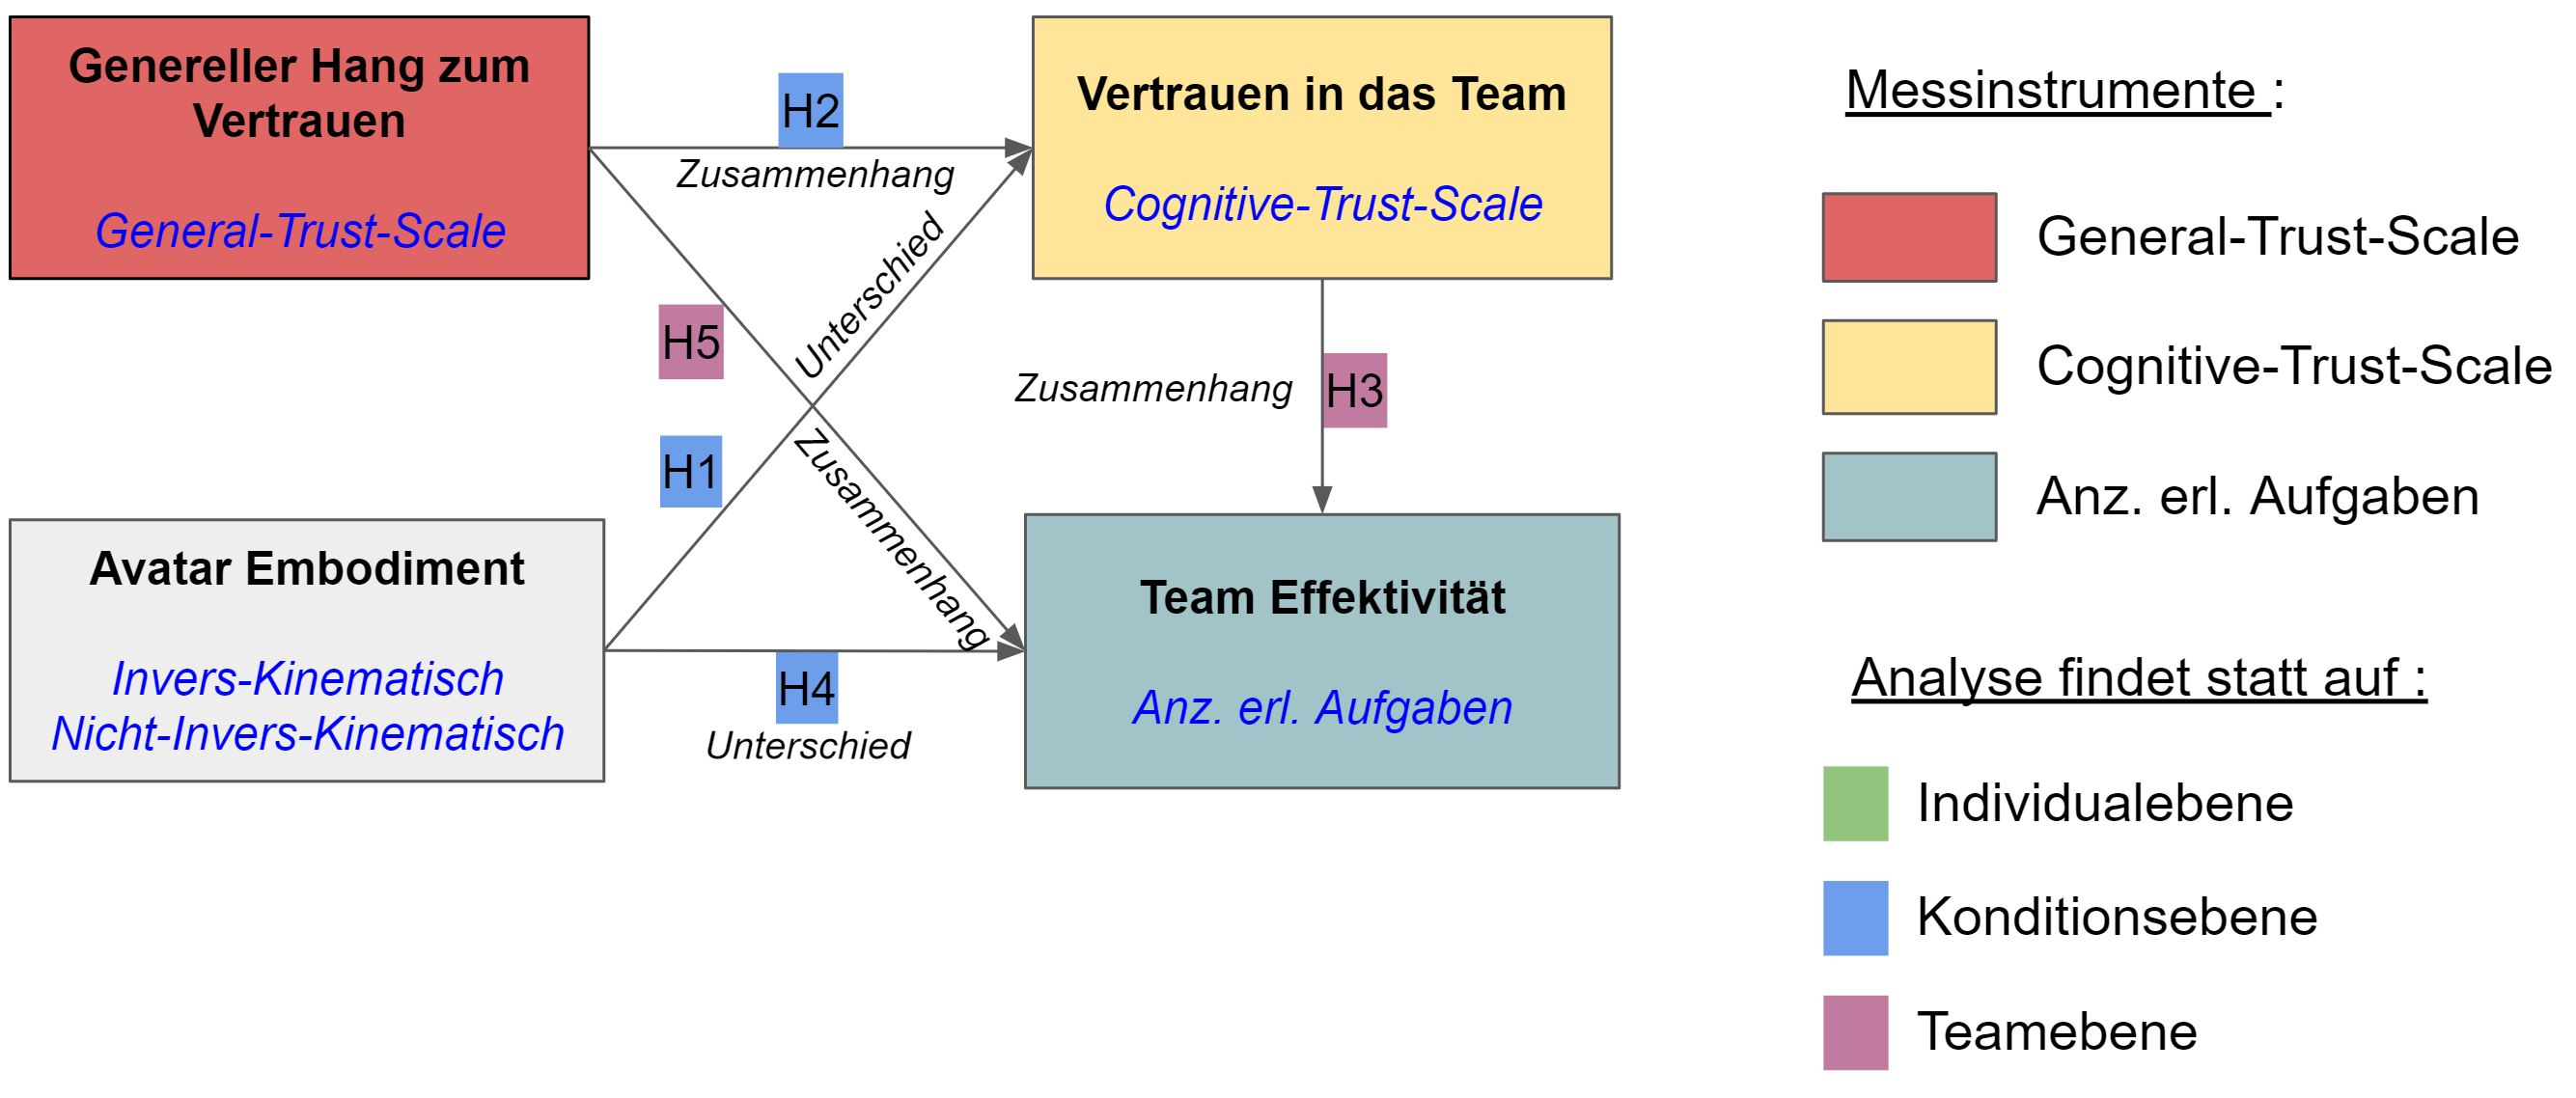
\includegraphics[width=\linewidth]{Abbildungen/Versuchshypothesen_02.JPG}		
			\caption[The self-constructed framework of experimental hypotheses]{This framework illustrates the interrelationships of the posed hypotheses.}
			\label{Versuchshypothesen}
		\end{footnotesize}
	\end{figure}	

General trust in this study refers to the extent to which participants tend to give others the benefit of the doubt. \citep{mcallister1995affect}.
\textit{Cognitive trust} refers to \textit{conviction} in the abilities or in the reliability of another \citep{mcallister1995affect}.
The \textit{team effectiveness} is measured by the number of rounds completed by the team during the experiment.

\begin{table*}
  \caption{MEASURING METHODS}
  \label{questionnaires}
  \begin{tabular}{llcr}
    \toprule
    Scale & What was measured? & $\alpha$ & Likert-Points \\
    \midrule
    \texttt{General-Trust-Scale \citep{couch1996assessment}} & Propensity to trust of the individual participants & ,91 & 1-7 \\
    
    \texttt{Cognitive-Trust-Scale \citep{mcallister1995affect}} &Built up cognitive trust during the experiment & ,91 & 1-5\\
    
     \texttt{\textit{Quality of team communication} \citep{gonzalez2014climate}} & Perceived quality of team communication & ,76 & 1-5 \\
     
      \texttt{\textit{Perceived team effectiveness}\citep{gibson2003team}} & Extent of the perceived team effectiveness & ,62-,88 & 1-7\\
          
       \texttt{NASA-TLX\citep{NASATLX}} & Task load during the experiment & ,84 &1-21  \\
       
       \texttt{IPQ \citep{IPQ}} & The sense of presence & ,85 & 1-7 \\
       
        \texttt{\textit{Co-Präsenz} \citep{nowak2003effect}} &  Co-, Social-, Telepresence & ,78-,90 & 1-7; 1-10 \\
    \bottomrule
  \end{tabular}
\end{table*}

\subsection{PARTICIPANTS}

The participants were acquired in two ways. Firstly, people in the circle of acquaintances were approached, who would be provided with the necessary hardware. Secondly, participants were sought in various forums (e.g. VRForum.de, Computerbase.de, Hardwareluxx.de, etc.). Furthermore, participants were acquired with the help of various social networks related to VR, as well as random Social Network chat groups with 50 or more members.

To participate in the experiment, participants required a fully functioning SteamVR, Windows Mixed Reality, or Oculus Rift/Rift-S Head-Mounted Display with compatible controllers, as well as a powerful VR-capable Computer. The leader of the experiment used a Computer without a Head-Mounted-Display, to control and manage the experiment from the outside.

\subsection{PROCEDURE AND IMPLEMENTATION}
To conduct the experiment a shared virtual environment was developed, in which three team members could see and interact with each other as avatars. During the experiment, the participants had to recognize different symbols by interacting with each other in order to advance to higher rounds as a team. The shared virtual environment has been developed with Unity 2019.4.3f1 and the HD render pipeline. To ensure real-time communication between clients the multiplayer framework \textit{Normcore v2.0}\footnote{www.Normcore.io} was used.
\textit{Figure \ref{AvatareImEinsatz}} shows both avatar conditions \textit{humanlike} (a) and \textit{non-humanlike} (b) during the experimental procedure in the Shared Virtual Environment.

Three people were placed in each time slot to form a team. The participants were \textit{not} introduced face-to-face and they saw themselves only as a representation of an avatar.
The test lasted 35 minutes and was divided into:
		\begin{itemize}
			\item 5 minutes pre-questionnaire,
			\item 5 minutes video explanation,
			\item 10 minutes experiment,
			\item 15 minutes post-questionnaire.
		\end{itemize}
The pre-questionnaire was used to collect general demographic data about the participants. The video explanation showed all the relevant mechanics of the experiment. Furthermore, it ensured that all participating individuals had the same level of information about how the experiment was conducted. During the experimental session, participants had 10 minutes to complete the collaborative task. Over the subsequent post-questionnaire, all relevant questionnaires shown in \textit{Table \ref{questionnaires}} were completed for later statistical analysis of the experimental hypothesis. The duration of the experiment was 600 seconds and a maximum of 15 rounds could be completed. The rounds increased incrementally in difficulty every third round, as one symbol was added to the pool of symbols to be guessed.
\textit{Figure \ref{RoundDifficulty}} shows the increasing round difficulty used to measure \textit{team effectiveness} in this experiment.

\begin{figure}[H]
		\begin{footnotesize}
		\centering
			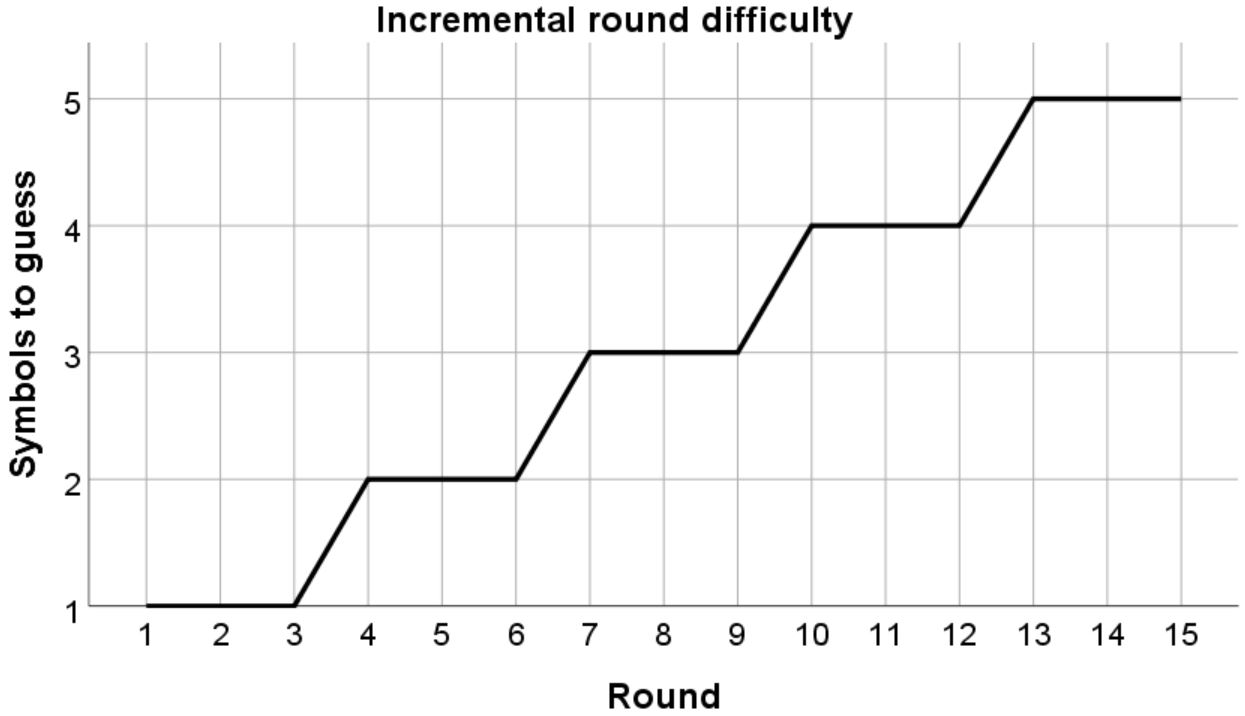
\includegraphics[width=0.9\linewidth]{Abbildungen/RoundDifficulty.JPG}	
			\caption[The difficulty of the rounds]{The increasing difficulty of the symbols to be guessed after each round. In round 1-3 one symbol had to be guessed, in round 3-6 two symbols and so on.}
			\label{RoundDifficulty}
		\end{footnotesize}
	\end{figure}

%\subsection{DETAILED TEST EXECUTION}
%At the beginning of each new round, players were assigned the color black, green or red.
%The player marked black had the task of explaining to his teammates the symbols that are color-coded for him. The other team members had the task to identify the symbols shown by the black player by gesticulation and to log them on their podium. The goal was to correctly identify as many symbols as possible, thereby advancing to following rounds together. %Check
%
%The symbols on the podium of the player marked in black were color-coded either green, red or green-red. The podiums of the other players also had the same symbols on them, but these were arranged randomly and had no color markings. The player marked in black had to explain the symbols marked in the respective player color in front of him to the other players marked with red and green. If the player who just had got addressed by the black player believed to have recognized a symbol, he logged the symbol by pressing down the matching button on his podium. 
%
%If all the marked symbols were successfully identified and logged in, a bright green ball appeared, indicating the end of the round.
%In the next round, another player was marked with black, red or green.

	
\begin{figure}[H]
  \centering
  \subfloat[][]{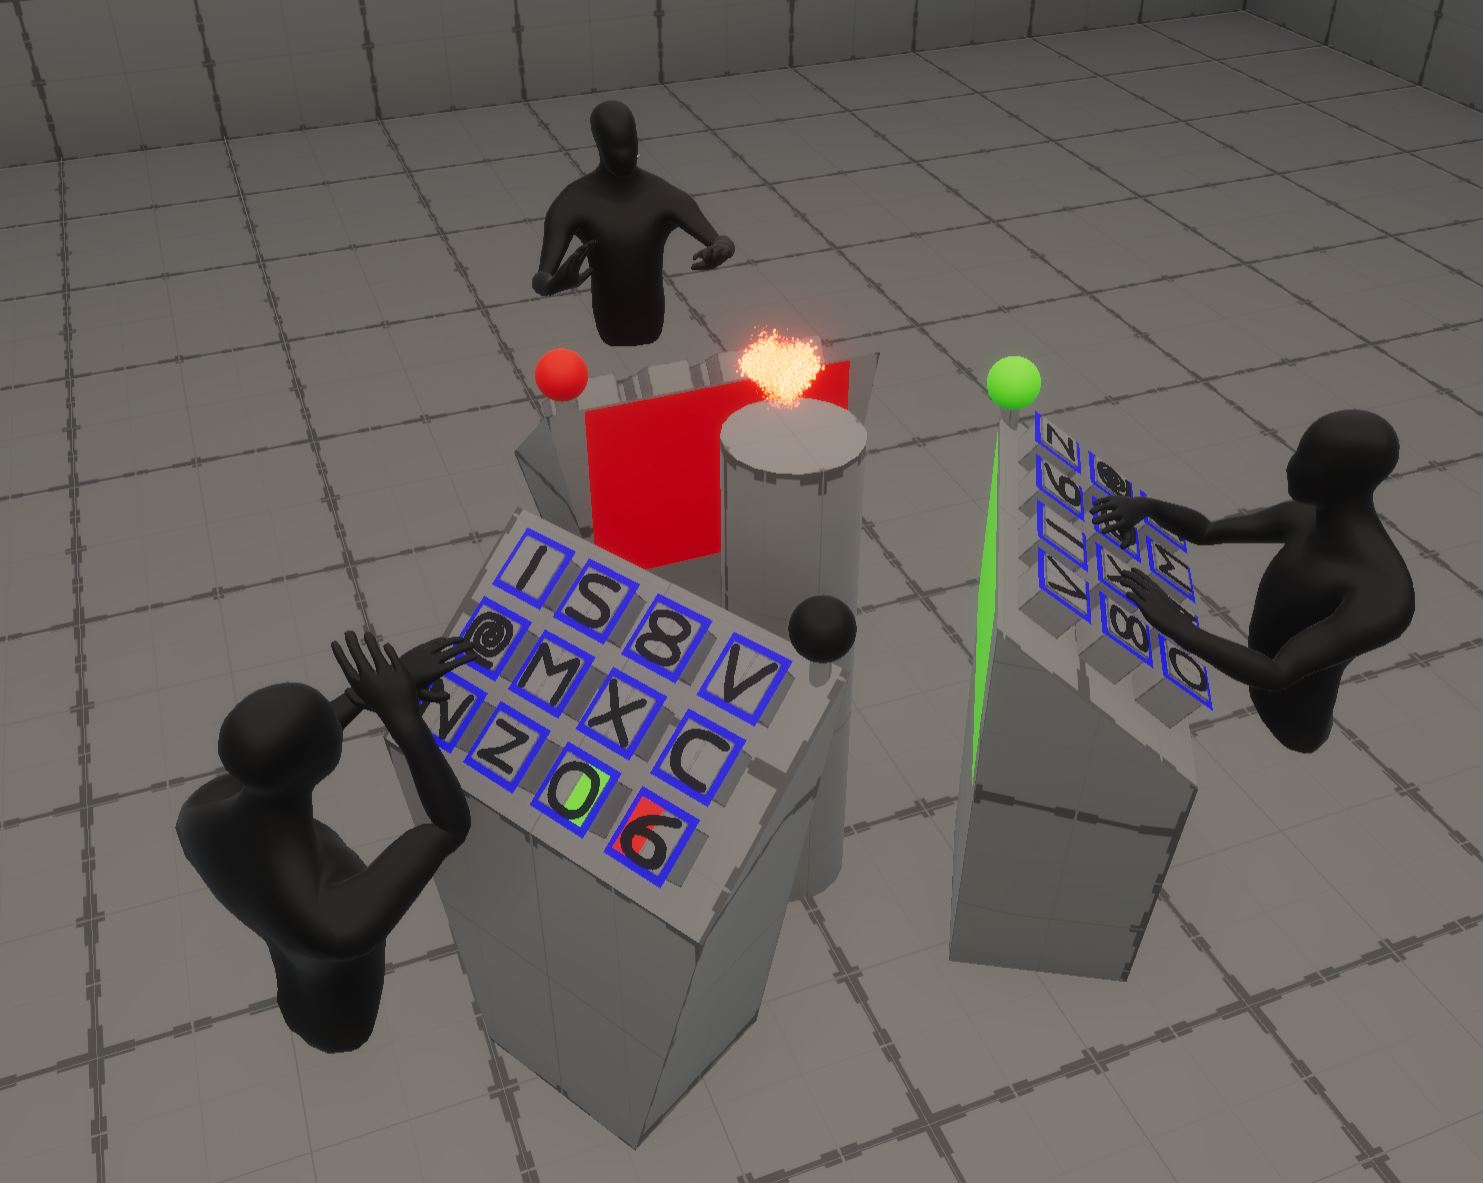
\includegraphics[width=0.41\linewidth]{Abbildungen/Podeste_IK_Avatars.jpg}}
  \qquad
  \subfloat[][]{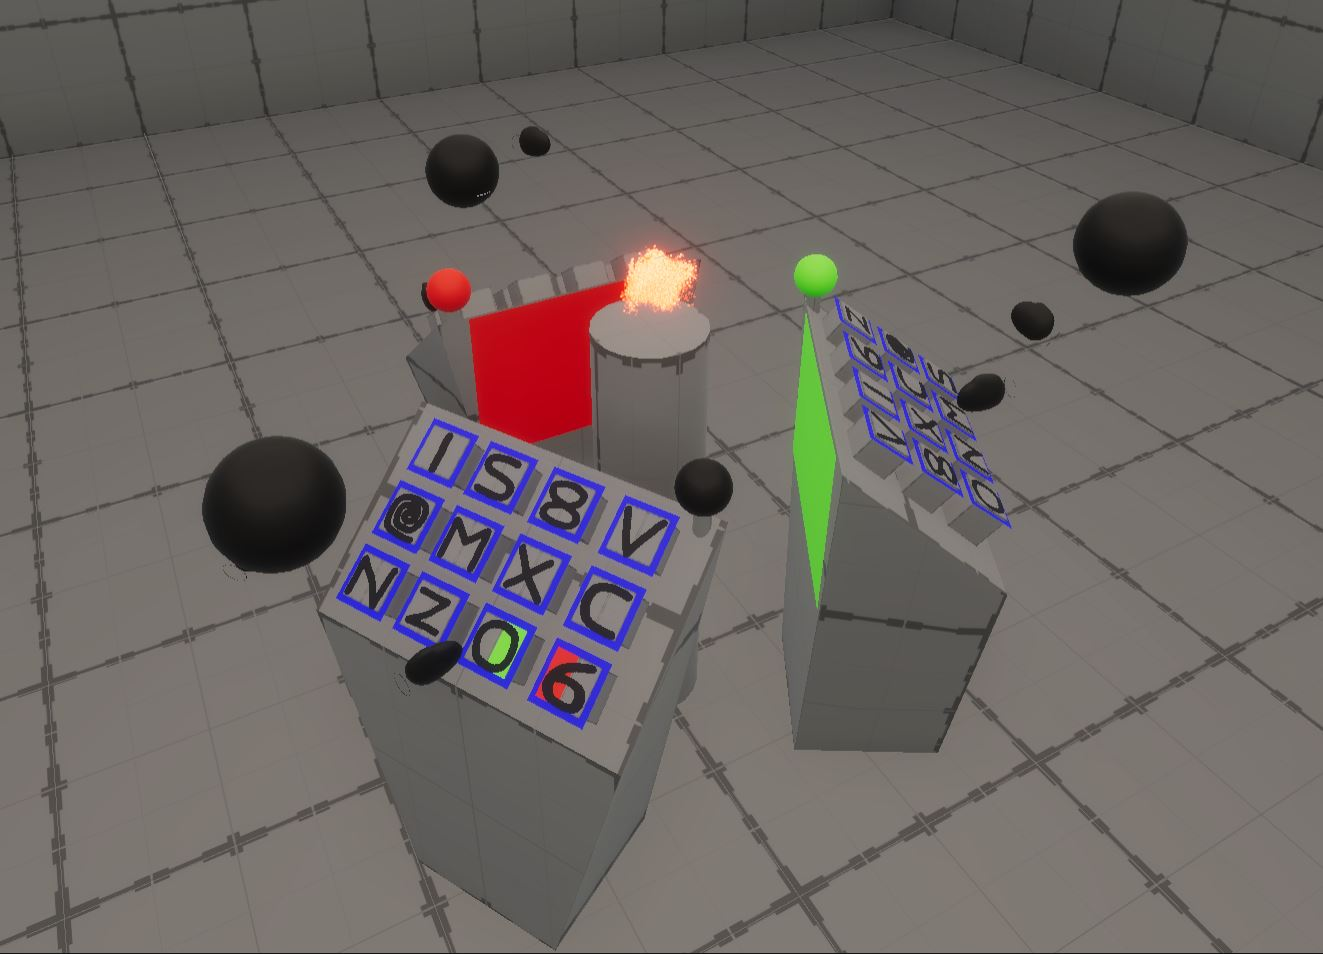
\includegraphics[width=0.45\linewidth]{Abbildungen/Podeste_Non_IK_Avatars.jpg}}
  \caption[The avatars in the experimental environment]{Avatar conditions \textit{humanlike} (a) and \textit{non-humanlike} (b) during the execution of the experiment. The color-coded symbols of the black-marked player can be seen on his podium.}
  \label{AvatareImEinsatz}
\end{figure}

\begin{table*}
  \caption{HYPOTHESIS ACCEPTED OR REJECTED}
  \label{AcceptOrReject}
  \begin{tabular}{ll}
    \toprule
    Hypothesis & Accepted? \\
    \midrule
     \texttt{Hypothesis 1} & \textbf{Accepted} \\
     \texttt{Hypothesis 2} & Rejected \\
     \texttt{Hypothesis 3} & Rejected \\
     \texttt{Hypothesis 4} & Rejected \\
     \texttt{Hypothesis 5} & Rejected \\
    \bottomrule
  \end{tabular}
\end{table*}

\section{RESULTS}
A total of 30 people participated in the study, forming a total of ten teams. Nineteen (63.3\%) individuals were male and 11 (36.7\%) were female. On average, participants were 30 years old $(\bar{x} = 30.13)$, with the second quartile being $28$ years old. % Check

Before the results were analyzed, a Shapiro-Wilk significance test was performed to check for normality.

\subsection{HYPOTHESIS}
%H1
Based on the statistical analysis of hypothesis 1 on \textit{condition level}, it can be concluded that different avatar conditions have a \textit{significant} influence on the formed \textit{cognitive trust} (Mann-Whitney-U: $U = 64.000; Z = -2.029; p =.042 < \alpha =.05; r =-.370$). Thereby, participants with the condition \textit{non-humanlike} $(\bar{x} = 4.622)$ formed more \textit{cognitive trust} than participants with the condition \textit{humanlike} $(\bar{x} = 4.188)$ (see \textit{Figure \ref{H1H4} (a)}). 

%H2
Through the analysis of hypothesis 2 on \textit{condition level}, \textit{no evidence} was found that there is a \textit{significant} correlation between \textit{general trust} and \textit{cognitive trust} (see \textit{Figure \ref{H2H3H5} (a) and (b)}). 

%H3
Contrary to the assumption of hypothesis 3, a \textit{significant} relationship was found between the formed \textit{cognitive trust in the team} and the \textit{team effectiveness} with the condition \textit{non-humanlike} \textit{on team level} (Spearman-Rho: $r =.975$; $p =.005 < \alpha = .05$). According to Fisher Z-score for independent samples \citep[p. 109]{cohen2013statistical} this correlation is \textit{significantly} different ($Z=-1.977$; $p =.024 < \alpha = .05$) from that correlation of the condition \textit{humanlike} (see \textit{Figure \ref{H2H3H5} (c) and (d)}).
 
%H4
During the analysis of hypothesis 4 on \textit{condition level}, it was found that the mean values of the obtained \textit{team effectiveness scores} are \textit{not significantly} different from each other due to different avatar conditions (Mann-Whitney U: $U = 103.500; Z = -.377; p =.706 > \alpha = .05; r = -.060$). An average team effectiveness of $\bar{x} = 9$ was found for both avatar conditions (see \textit{Figure \ref{H1H4} (b)}).

%H5
Based on the analysis of hypothesis 5 on \textit{team level}, there is \textit{no evidence}, that there is a \textit{significant} correlation between a person's \textit{general trust} and \textit{team effectiveness} in a \textit{virtual team} (see \textit{Figure \ref{H2H3H5} (e) and (f)}).

\textit{Table \ref{AcceptOrReject}} shows, whether a hypothesis was accepted or rejected.


\begin{figure}[H]
  \centering
  \subfloat[][]{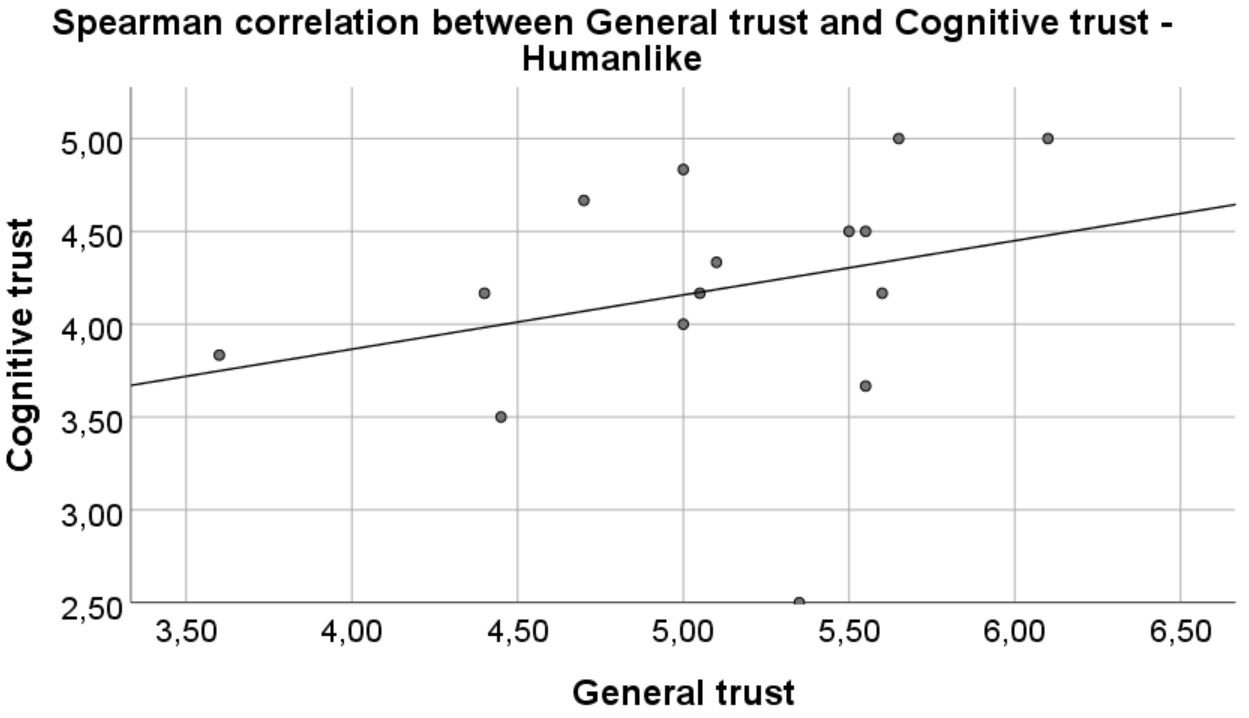
\includegraphics[width=0.46\linewidth]{Abbildungen/H2_Korr_IK.jpg}}
  \qquad
  \subfloat[][]{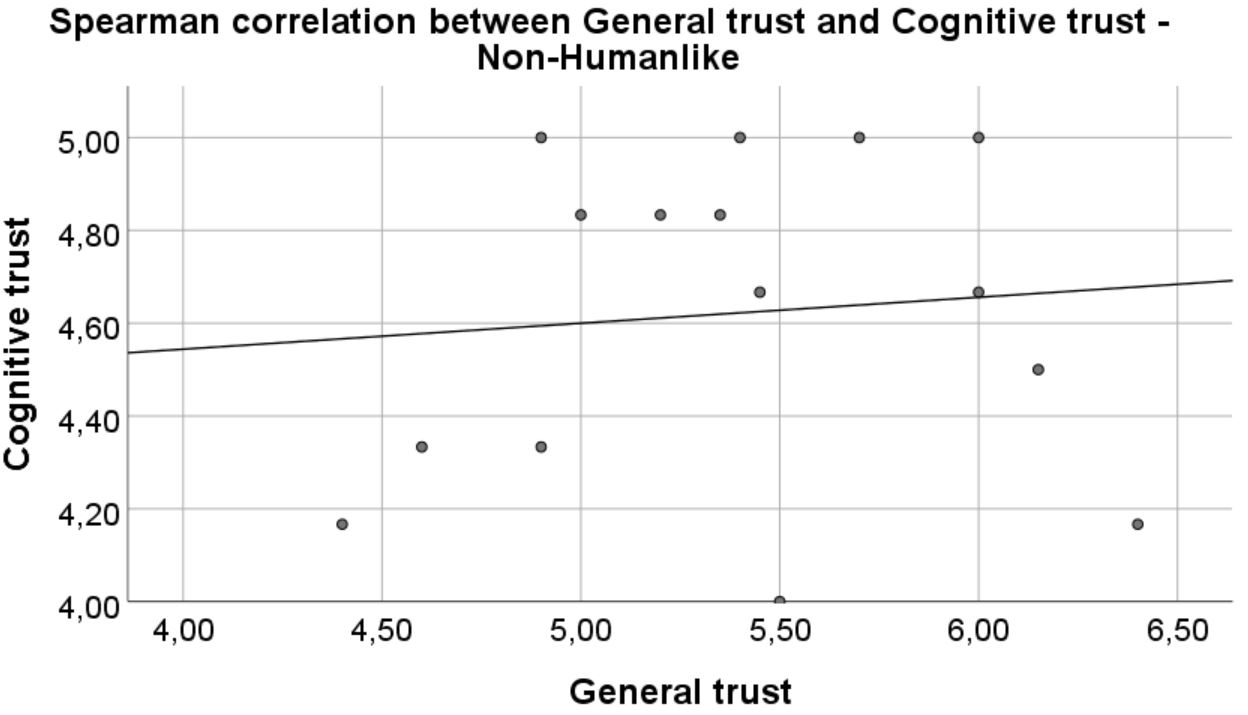
\includegraphics[width=0.46\linewidth]{Abbildungen/H2_Korr_NIK.jpg}}
  \qquad
  \subfloat[][]{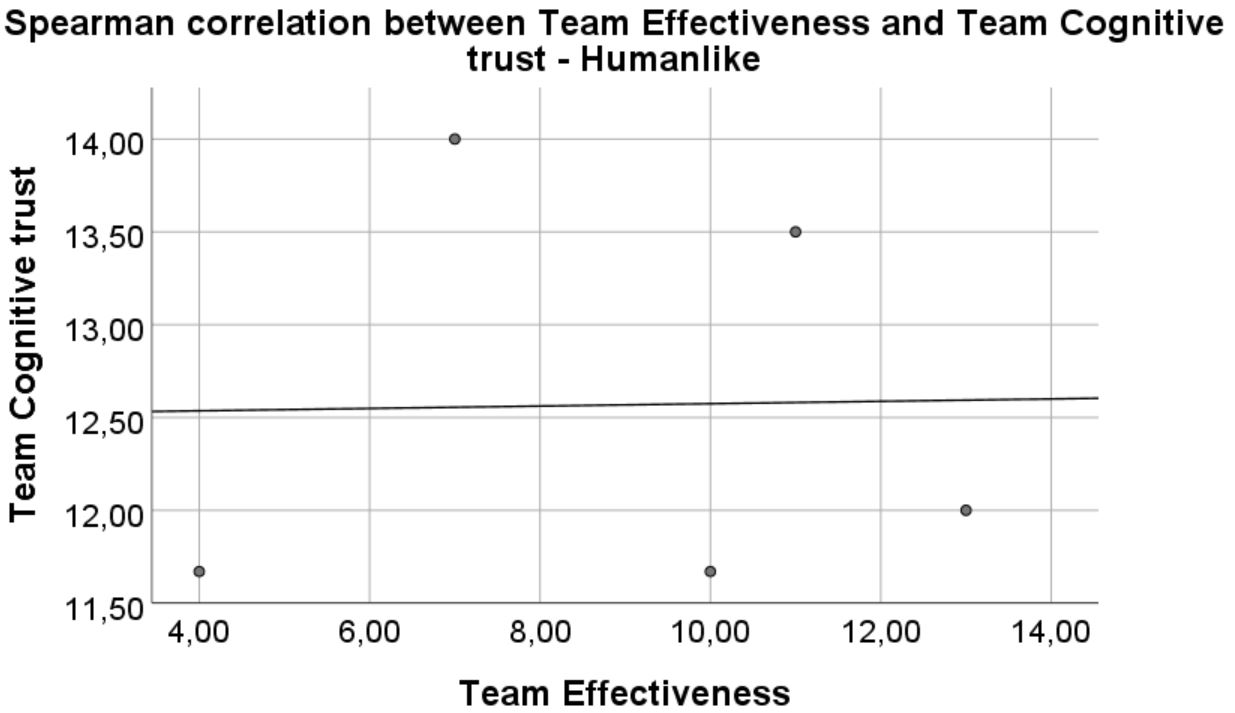
\includegraphics[width=0.46\linewidth]{Abbildungen/H3_Korr_IK.jpg}}
  \qquad
  \subfloat[][]{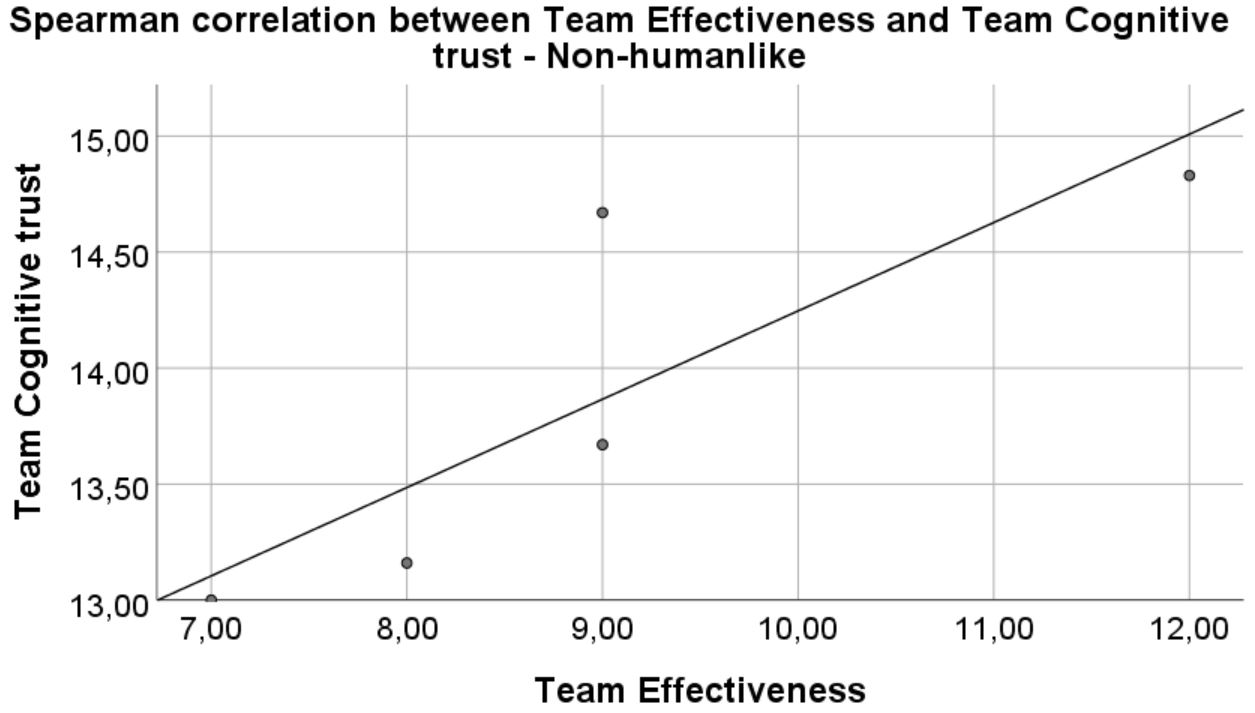
\includegraphics[width=0.46\linewidth]{Abbildungen/H3_Korr_NIK.jpg}}
  \qquad
  \subfloat[][]{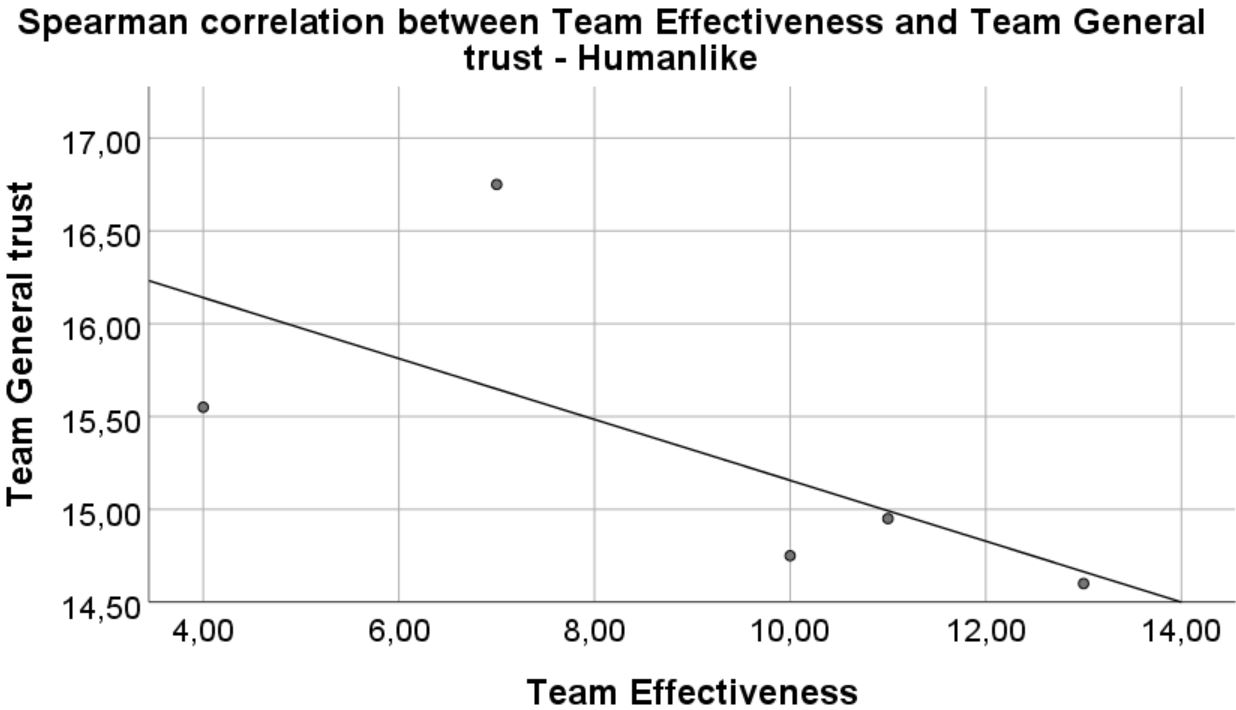
\includegraphics[width=0.46\linewidth]{Abbildungen/H5_Korr_IK.jpg}}
  \qquad
  \subfloat[][]{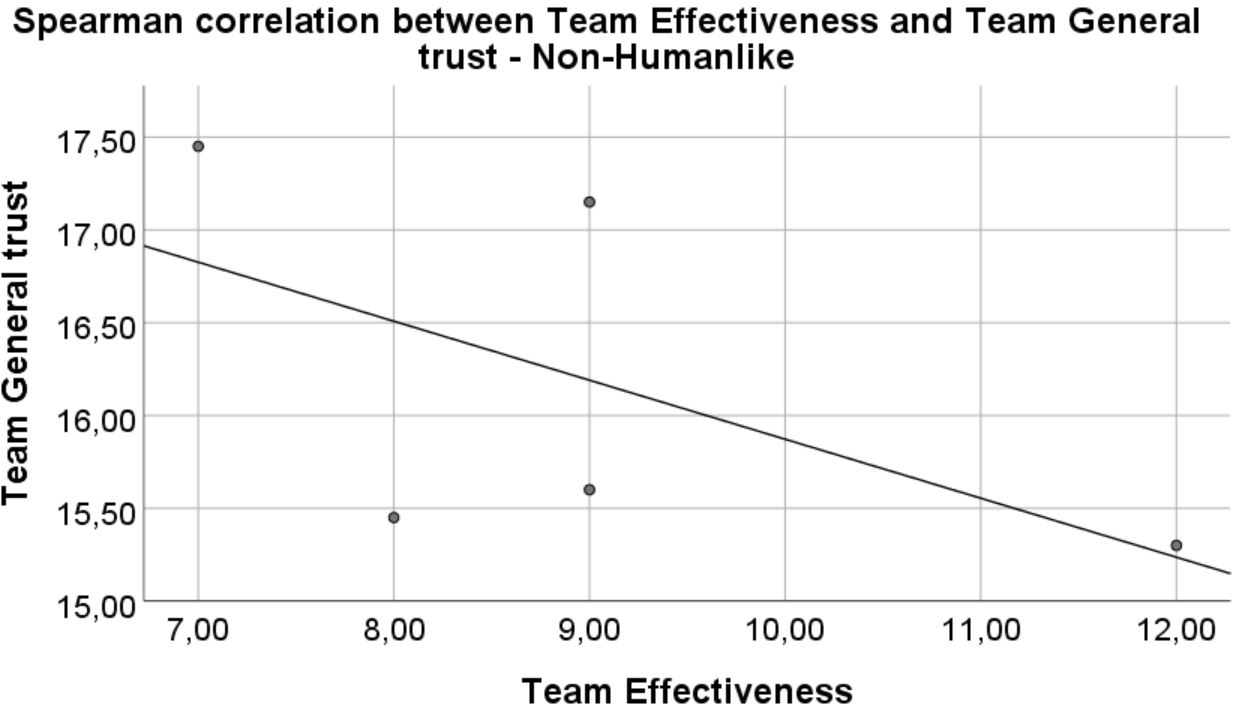
\includegraphics[width=0.46\linewidth]{Abbildungen/H5_Korr_NIK.jpg}}
  \qquad
  \caption[Results of hypothesis 2, 3 and 5]{Figure (a) and (b) show the results of hypothesis 2 on condition level. Figure (c) and (d) show the results of hypothesis 3 on team level. (e) and (f) show the results of hypothesis 5 on team level.}
  \label{H2H3H5}
\end{figure}

\begin{figure}[]
  \centering
  \subfloat[][]{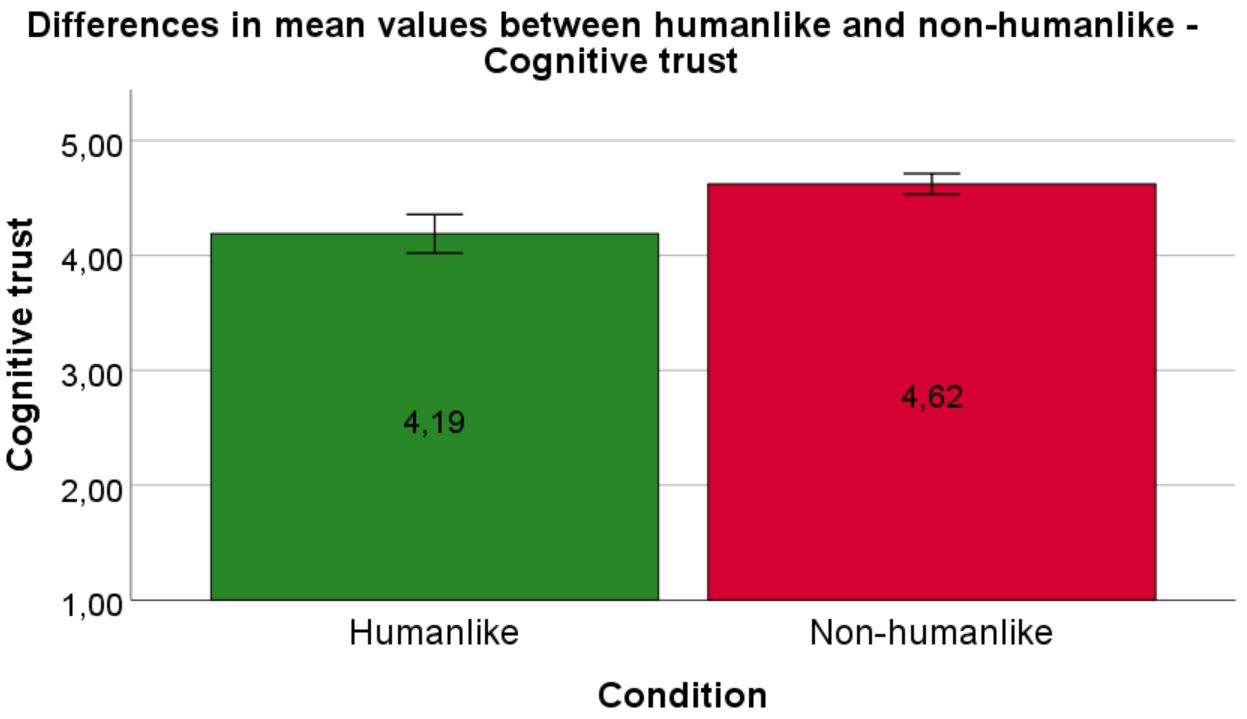
\includegraphics[width=0.8\linewidth]{Abbildungen/H1_Difference.jpg}}
  \qquad
  \subfloat[][]{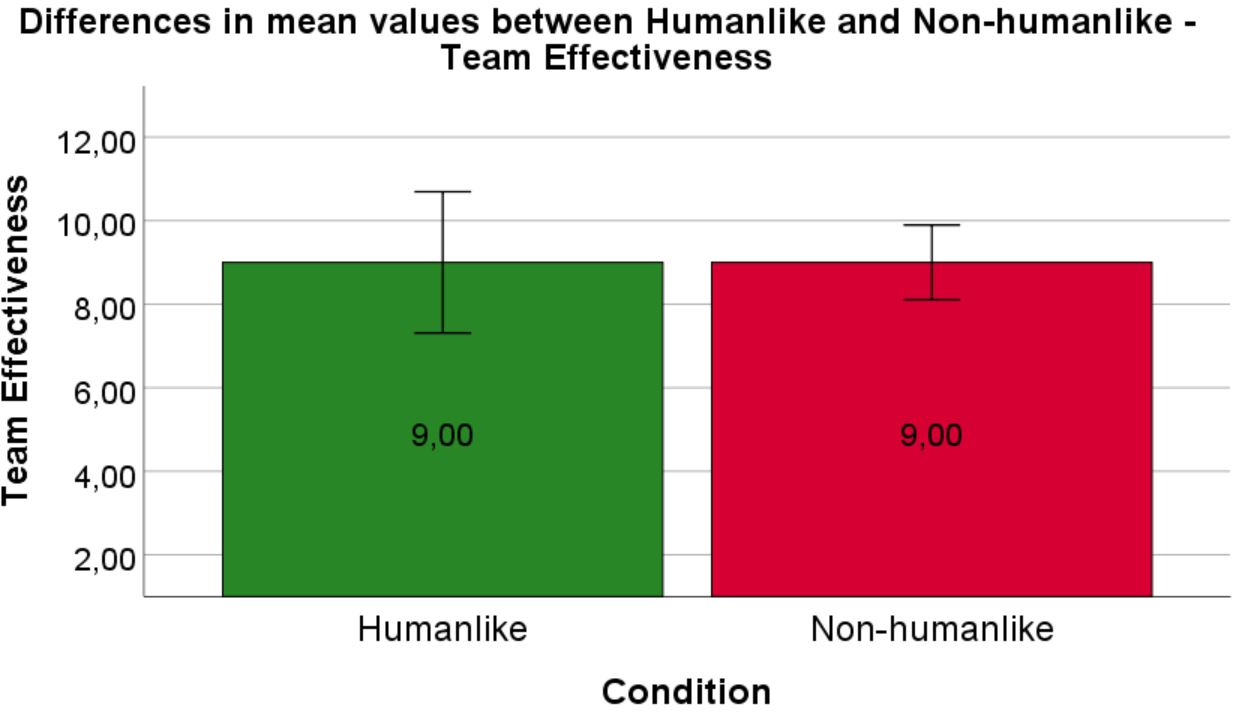
\includegraphics[width=0.8\linewidth]{Abbildungen/H4_Difference.jpg}}
  \caption[Results of hypothesis 1 and 4]{Figure (a) shows the results of hypothesis 1 on condition level. (b) shows the results of hypothesis 4 on condition level.}
  \label{H1H4}
\end{figure}

\newpage
\subsection{SUBJECTIVE DATA}
The analysis of the subjective data on the condition level shows, a \textit{significant} difference of the mean values of team communication (Mann-Whitney-U : $U = 63.500; Z = -2.062; p =.039 < \alpha = .05$). The mean value of the \textit{team communication} of the condition \textit{humanlike} is $\bar{x} = 4.013$, while for the condition \textit{non-humanlike} it is  $\bar{x} = 4.48$. For both conditions, the tendency of a high team communication is evident ($\bar{x} = 4.013$; $\bar{x} = 4.48$ $ > \bar{x} = 3$).

Furthermore, on condition level with the condition \textit{non-humanlike} a \textit{significant} positive correlation between \textit{cognitive trust} and \textit{perceived team effectiveness} was found (Spearman-Rho: $r =.869; p =.000 < \alpha = .05$) (see \textit{Figure \ref{SubDataCorr} (a)}).

Also, a \textit{significant} positive correlation with the condition \textit{non-humanlike} at the condition level between \textit{cognitive trust} and \textit{team communication} was found (Spearman-Rho: $r =.676; p =.006 < \alpha = .05$) (see \textit{Figure \ref{SubDataCorr} (b)}).

Moreover, it can be noted that an increased sense of presence (presence ($\bar{x} = 4.446 > \bar{x} = 3.5$), telepresence ($\bar{x} = 4.446 > \bar{x} = 3.5$), self-perceived co-presence ($\bar{x} = 3, 827 > \bar{x} = 2.5$), perceived co-presence of the other ($\bar{x} = 3.877 > \bar{x} = 2.5$), and social presence ($\bar{x} = 6.409 > \bar{x} = 5$)) was formed on individual level during the experiment. Overall the perceived stress level was below average ($\bar{x} = 7 < \bar{x} = 11$) and perceived team effectiveness was above average ($\bar{x} = 4.886 > \bar{x} = 3.5$).

\textit{Table \ref{SubDataSigs}} shows, whether a significant difference was found by analyzing the subjective data.

\begin{table*}
	\caption{SIGNIFICANCE OF SUBJECTIVE DATA ANALYSIS}
  \label{SubDataSigs}
  \begin{tabular}{ll}
    \toprule
    What was measured? & Significance found? \\
    \midrule
     \texttt{Presence} & no significant difference \\
   	 \texttt{Self-perceived co-presence} & no significant difference \\
     \texttt{Perceived co-presence of the other} & no significant difference  \\
     \texttt{Telepresence} & no significant difference \\
     \texttt{Social presence} & no significant difference \\
     \texttt{Perceived stresslevel} & no significant difference \\
     \texttt{Team communication} & \textbf{significant difference} \\
     \texttt{Perceived Team effectiveness} & no significant difference  \\
    \bottomrule
  \end{tabular}
\end{table*}

\begin{figure}[]
  \centering
  \subfloat[][]{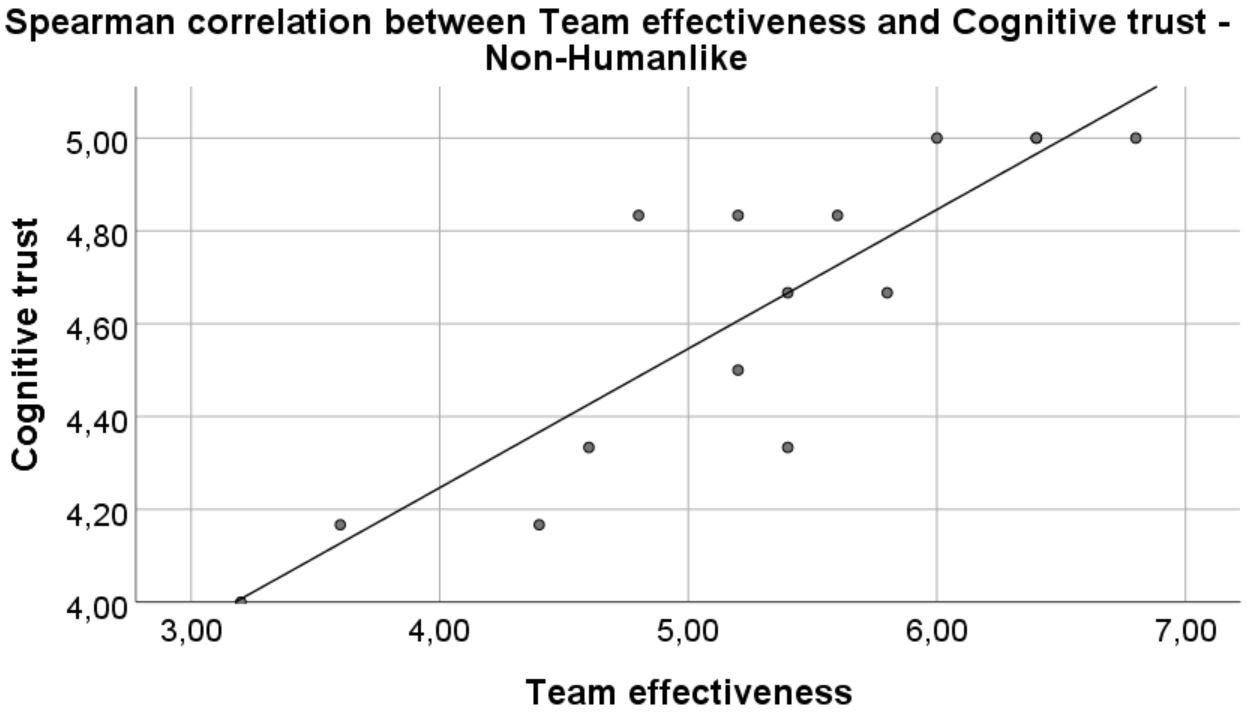
\includegraphics[width=0.46\linewidth]{Abbildungen/SubDataTE.jpg}}
  \qquad
  \subfloat[][]{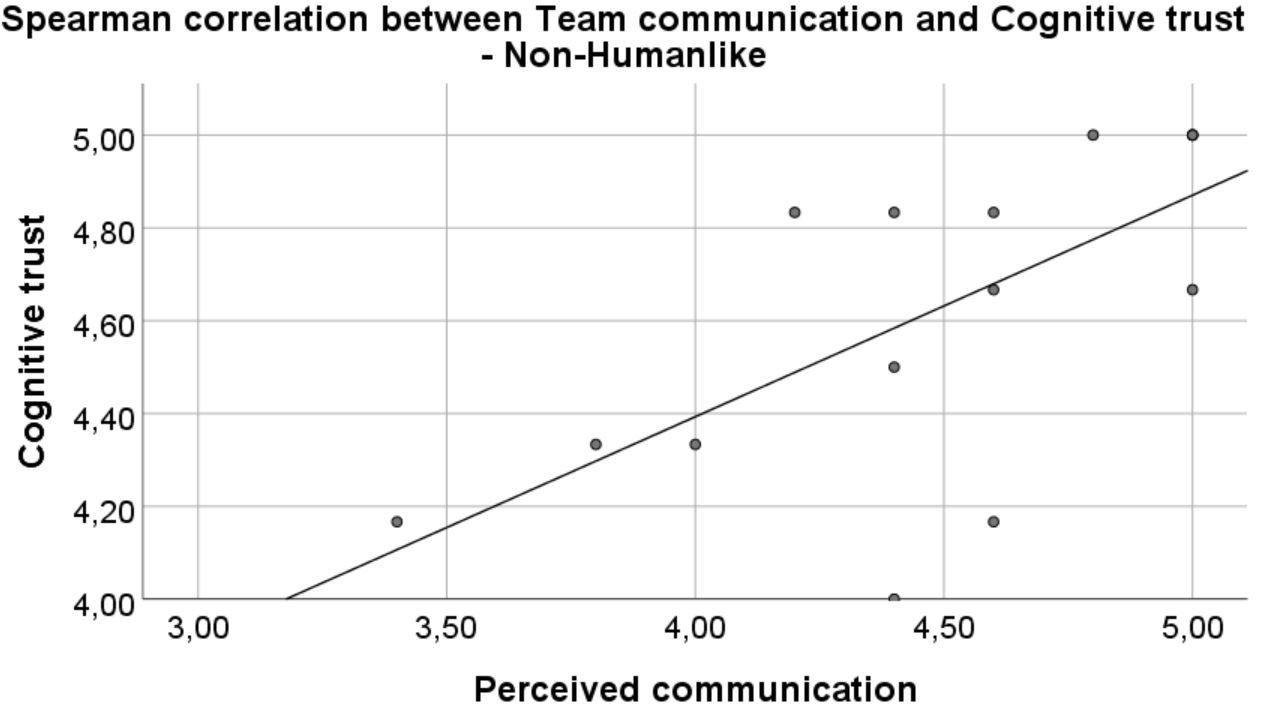
\includegraphics[width=0.46\linewidth]{Abbildungen/SubDataTC.jpg}}
  \caption[Significant correlations Cognitive trust, Team effectiveness and Team communication]{Figure (a) shows the significant correlation of the condition non-humanlike between the perceived team effectiveness and cognitive trust. Figure (b) shows the significant correlation of the condition non-humanlike between perceived team communication and cognitive trust. }
  \label{SubDataCorr}
\end{figure}

\section{DISCUSSION}
In this chapter, the results of the study are discussed and limitations are pointed out.

\subsection{BUILDING COGNITIVE TRUST THROUGH DIFFERENT AVATAR CONDITIONS}
The results of hypothesis 1 contradict the study by Bente et al. \citep{bente2004social}, which suggested that there is a greater increase of \textit{cognitive trust} with the condition \textit{humanlike} than with the condition \textit{non-humanlike}. According to the statistical analysis the opposite was the case in this study, because the participants with the condition \textit{non-humanlike} achieve on average a significantly higher \textit{cognitive trust} score.
One reason for this result could be that the used \textit{humanlike} avatar was affected by the \textit{Uncanny Valley Effect}\footnote{The Uncanny Valley Effect describes the feeling of uneasiness above a certain level of reality \citep[p. 352-353]{guest2011uncanny}.}.
Furthermore, the inverse kinematics used in this experiment could have been perceived as strange due to the inverse-kinematics used. Misinterpreted gesticulation may also have led to a lower level of trust in the \textit{humanlike} condition. It is assumed that the simplicity of the \textit{non-humanlike} avatar condition is easier to adopt in a short timeframe of collaboration.

\subsection{BUILDING COGNITIVE TRUST THROUGH GENERAL TRUST}
The fact that there is no significant correlation between \textit{cognitive trust} and \textit{general trust} with different avatar conditions (hypothesis 2) can also be seen as an advantage.
Thus, it can be supposed that during short-term collaboration in a shared virtual environment it is not relevant how high or low a person's \textit{baseline of trust} is. 
Since only the different avatar conditions have a significant impact on the formation of cognitive trust, it can be assumed that \textit{general trust} does not play a major role during a get-to-know phase of a virtual team and can be considered separately. %Check can be ignored? 

\subsection{TRUST IN THE TEAM AND TEAM EFFECTIVENESS}
Since hypothesis 4 cannot be accepted, but a significant correlation with the condition \textit{non-humanlike} was found in the analysis of hypothesis 3, it must be suspected that the results of hypothesis 3 and hypothesis 4 are either random in nature, the measurement of team effectiveness needs to be improved or that cognitive confidence had no effect on team effectiveness.
The small sample size of the study could also be a reason why the results of hypothesis 3, hypothesis 4 and hypothesis 5 do not provide clear results. With a significantly larger sample size, a significant difference (hypothesis 4) or a clear significant correlation between the build \textit{cognitive trust} and the \textit{team effectiveness} (hypothesis 3), if any, could be found with a larger variance of the \textit{team effectiveness} scores obtained.

\subsection{LIMITATIONS}
One technical limitation of this work is the technique used for gesticulation. The supported head-mounted displays did not offer the possibility to display the fingers or the whole hands in virtual reality since it was observed that participants with the condition \text{humanlike} wanted to express themselves more than it was possible. The communication within the shared virtual environment can be intensified by using finger and hand tracking to create a higher degree of realism. Another aspect to increase human likeness in the \textit{humanlike} avatar condition would be the use of facial expressions.
Another limitation of this study is that participants knew that they would interact with real people. %Check instead of bots?

\section{CONCLUSION AND FUTURE WORK}
The goal of this study was to investigate the impact of two different avatar conditions (humanlike and non-humanlike) on \textit{team trust} formation and the resulting \textit{team effectiveness} in a shared virtual environment. 

For the experiment three spatially separated participants simultaneously had to complete tasks as a team in a shared virtual environment. Each team was assigned to one of two different avatar conditions. While performing the mutual task, the collaborative \textit{team effectiveness} was determined. The questionnaire survey was used to gain insight into \textit{general trust} and \textit{cognitive trust} formed, as well as the \textit{perceived team effectiveness}, the \textit{subjective feelings} regarding workload and the \textit{feeling of presence} formed.

Shared virtual environments are currently developing rapidly. The corona pandemic has shown that virtual collaboration efforts are having a major impact on businesses worldwide. More research is needed on how teams can collaborate effectively in a shared virtual environment.

Not only could be studied which type of avatar in a shared virtual environment creates more \textit{trust} or generates more \textit{team effectiveness}, but also how language, facial expressions, gestures, size, gender, or prior familiarity of the subjects affects these variables.
Furthermore, it could be investigated how the duration of head-mounted display use affects team trust and team effectiveness.

A follow-up to this study could investigate the extent to which \textit{cognitive trust formation in the team} changes, depending on whether participants know that they are collaborating with humans or not. In addition, it would be of interest to investigate how much the difference between verbal and a nonverbal communication affects the formed trust in the team.  
Furthermore, similar studies could be conducted in which the individual rounds of the collaboration task are executed faster one after the other or in which the avatars have a different appearance.

Overall, a significant difference in formed \textit{cognitive trust} was found between the avatar conditions, with more \textit{cognitive trust} formed with the \textit{non-humanlike} condition. A significant relationship was found between \textit{cognitive trust} and \textit{team effectiveness} with the condition \textit{non-humanlike}. However, no statistically significant difference was found between avatar conditions and \textit{team effectiveness}. The results also show no significant correlation between a person's \textit{general trust} and formed \textit{cognitive trust}. Furthermore, there is no significant correlation between \textit{general trust} and \textit{team effectiveness}.

Thus, in a virtual team, according to this study, the avatar condition has no clear influence on \textit{team effectiveness}. The \textit{general trust} does not affect the formation of \textit{cognitive trust} nor does it affect the \textit{team effectiveness}. However, it may be useful, not to make the avatar too humanlike in order to build more \textit{cognitive trust}.

Consequently, working in a virtual team does not have to be supported with complex avatars. For example, companies that want to work with virtual teams in a shared virtual environment can use simple avatar models to help building up trust within the team to be more effective.

%%
%% The next two lines define the bibliography style to be used, and
%% the bibliography file.
%\citestyle{acmauthoryear}
\bibliographystyle{ACM-Reference-Format}

\bibliography{sample-base-noDOI}

%%
%% If your work has an appendix, this is the place to put it.
\appendix


\end{document}
\endinput
%%
%% End of file `sample-sigconf.tex'.
